\section{Introduction}
\label{sec:intro}

The goal of this report is not to present a full overview of the state of the art in (large scale) computer vision and image processing (CV\&IP). It aims at identifying areas of expertise in CV\&IP whcih are required or exected to be required in e-science projects at NLeSc. From projects and proposals at NLeSc, where the data for the object of scientific research are captured as 2D/3D images, three main applications of CV\&IP  can be identified:
\begin{enumerate}
\item {\bf Where is my object? (Localization)} The problem is how to automaically find the subject of interes or reduce the data, sothey contain the subject of interest in large collections of images/videos.
\item {\bf What is my object? (Classification)}  The problemis to (semi-) automatically classify the study object to one of possbile categories. Usually the same equipment andmodality is used?
\item {\bf Is my object the same? (Identification)} The problem is to (semi-) automatically determine if the study subject is the same in multiple instatnces of photographic it, usually subject to differnt time, environment, viweing conditions or camera equipment.  
\end{enumerate}

For example in the systems biology project \href{https://blog.surf.nl/en/eyr4-blog-5-using-big-data-solutions-to-understand-worm-behavior/}{``Using big data solutions to understand worm behavior''}, the subject of reserach is the {\em C.elegans} worm (see Figure \ref{fig:Celegans}). The source data are high resolution and long videos caputing the behaviour of the worm. The first step is to {\em localize} precesely the worm in the large volume of imaging data. 
\begin{figure}[H]
\begin{center}
\includegraphics[width=0.8\textwidth]{fig/Celegans}
\end{center}
\caption{ Analysis of behavioural videos of C.elegans.}
\label{fig:Celegans}
\end{figure}
This is a good example of how the object of interest is often studied in controlled environment and one can assume that the most prominent (aka salient) object capruted on images/videos is the object of interest.In this case, the lab plate ensures relatively unifrom background where one can easiliy find the object of interest (the worm). The challage is tofind it automatically and to process efficiently large amounts of data.

The localisation problem is often related to the segmentation problem, which is most challenging in the medical imaging domain. Illustration of the difficulty of the problem can be seen in Figures \ref{fig:hippo} and \ref{fig:oct}.

\begin{figure}[H]
\begin{center}
\includegraphics[width=0.8\textwidth]{fig/hippo}
\end{center}
\caption{Hippocampus segmentation from an MRI subvolume. \href{https://www.esciencecenter.nl/project/biomarker-boosting}{BiomarkerBoosting project.}}
\label{fig:hippo}
\end{figure}


\begin{figure}[H]
\begin{center}
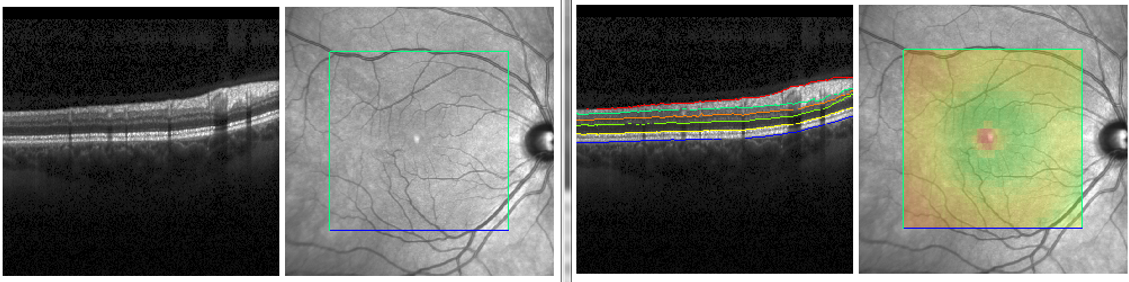
\includegraphics[width=0.8\textwidth]{fig/oct}
\end{center}
\caption{Optical Coherence Tomography (OCT) of retina layers segmentation: image data(left), image segmentation \& retina thickness map(right). \href{https://blog.surf.nl/eyr4-blog-7-lightpath-optical-coherence-tomography-oct-imaging/}{ EYR4 project: Lightpath for OCT imaging.}}
\label{fig:oct}
\end{figure}

Because of the large difficulty of the problem, the large number of imaging madalities and equipments usually special algorithms are develop to segment different body structures. Since specific solutions are required, they are hard to genneralize for other structures, modalities, less alone scientific domains, the image segmentaiton is left out of the scope of this report.

To address these application questions, three  CV\&IP research questions can be defined:
\begin{enumerate}
\item {\bf Visual salience:} How can the CV system determine automatically the most visual salient region(s) in an image?\label{item:sal}
\item {\bf Object/scene detection/classification:} How can the computer recognise automatically to what visual category the object/scene captured in an image belongs to? \label{item:und}
\item {\bf Object/scene identification:} How can the CV system automatically determine whether two images, potentially taken with different cameras under different viewing conditions and transformations, represent the same object/scene?\label{item:ident}
\end{enumerate}

There are also other numerous applications related to the above reserach  questions. For example visual saliency (\ref{item:sal}) in important in tasks such as:
\begin{itemize}
\item Automatic target detection (see fig. \ref{fig:sal})
\item Robot navigation using salient objects
\item Image and video compression
\item Automatic cropping/centering images for display on small portable screens
\item Tumor detection in mammograms, etc.
\end{itemize}

\begin{figure}[H]
\begin{center}
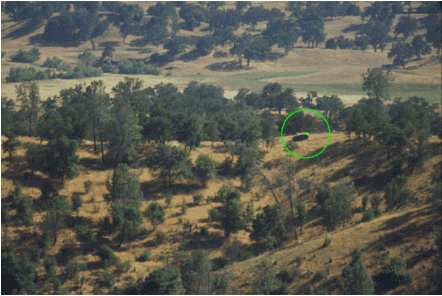
\includegraphics[width=0.8\textwidth]{fig/saliency}
\end{center}
\caption{Example of a saliency model detecting the vehicle as being the most salient object ina complex scene.}
\label{fig:sal}
\end{figure}

Few of the numerous applications related to object/scence identification (\ref{item:ident}) are:
\begin{itemize}
\item Stereo and wide-baseline matching
\item Image panorama stiching/creation
\item Automatic reconstruction of 3D scenes
\item Individual wildlife photo-identification (see figs.  \ref{fig:photoid} and \ref{fig:woodphotoid}), etc.
\end{itemize}

\begin{figure}[H]
\begin{center}
\includegraphics[width=0.8\textwidth]{fig/photoid}
\end{center}
\caption{Example species with sufficient spot pattering what could be useful for automated photo-identification: (a) whale shark (with reference area),
(b) spotted  tree frog, (c) northern quoll, (d) Amazon spotted frog, (e) striped blue crow and (f) mangrove snake.}
\label{fig:photoid}
\end{figure}

\begin{figure}[H]
\begin{center}
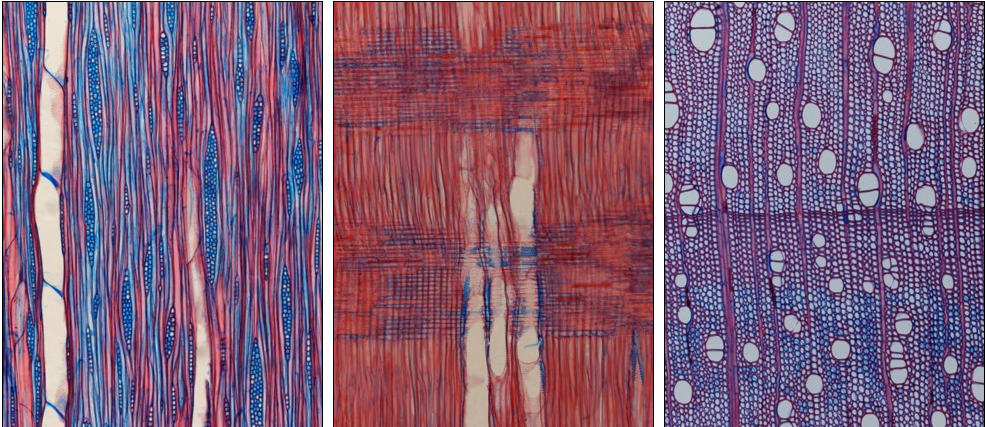
\includegraphics[width=0.8\textwidth]{fig/woodphotoid}
\end{center}
\caption{Left to right: tangential, radial and cross (transversal) sections of stained wood Acer.}
\label{fig:woodphotoid}
\end{figure}

Automatically understading the semantics of an object/scene (\ref{item:und}) have many applications like:
\begin{itemize}
\item Image search engines
\item Organizing photo collections
\item Autonomous driving
\item Human machine interaction, etc.
\end{itemize}

This is a complex and high-level computer vison task, with the goal of making machines see like humans and be able to infer both general principles as well as current situaitons from images. Example of a trained system for scee categorization is shown on fig.\ref{fig:mitdemo}.
\begin{figure}[H]
\begin{center}
\includegraphics[width=0.8\textwidth]{fig/mitdemo}
\end{center}
\caption{ \href{http://places.csail.mit.edu/demo.html}{MIT Scene Recognition Demo.}}
\label{fig:mitdemo}
\end{figure}

The overview is by no means complete, it rather tries to summarise the research in the field along the above three questions in the last years. 
These questions have been chosen having in mind the problems defined in other sciences whcih can be helped by computer science, more precisely by the developments in CV\&IP.

The report is structured along the three main products of CV\&IP reserach, namely, scientific publications in section \ref{sec:pubs}, software in section \ref{sec:soft} and datasets in section \ref{sec:db}. Each section gives examples of the work related to each of the three research questions. Some potential scientific aplications are shown in section \ref{sec:app}.

The goal of this report is not only to summarize, but is also an attempt to identify suitable "niche" for scientifical domain-driven (applied) research in CV\&IP at NLeSc. The conclusions and recommendations are given is section \ref{sec:conc}.